%----------------------------------------------------------------------------
\documentclass[11pt, t, beamer]{beamer}
%----------------------------------------------------------------------------
%% Versión para imprimir (modo artículo) %% Debes comentar el anterior comando \documentclass{}
%% Debes activar los cuatro comandos siguientes:

% \documentclass[12pt]{article} 
% \usepackage[]{beamerarticle}  
% \usepackage{graphicx}
% \usepackage[colorlinks]{hyperref}
%----------------------------------------------------------------------------
%% Paquetes generales necesarios

\usepackage[utf8]{inputenc}
\usepackage[T1]{fontenc}
\usepackage[spanish]{babel}
\usepackage{mathtools}  % Comandos ampliados en el entorno matemático
\usepackage{multirow} % Para unir filas en las tablas
\usepackage{listings} %Para resaltar de forma adecuada los comandos de R

\graphicspath{{./}{./eps/}{./jpg/}} %Directorios donde buscar las imágenes

%----------------------------------------------------------------------------
%% Información de la portada y de los marcos exteriores

\title%[Short Paper Title] % (optional, use only with long paper titles)
[Gráficos estadísticos (\insertframenumber/\inserttotalframenumber)]
	{Gráficos estadísticos}



\author[FGarcia]{
  Francisco García\\
  \href{mailto:fgarcia@cipf.es}{(fgarcia@cipf.es)}
}
% 
\institute[CIPF] % (optional, but mostly needed)
{
 CIPF's Research Development Programme
}

%----------------------------------------------------------------------------
%% Configuración de la versión para imprimir:
%%    - handout: para imprimir en papel y repartir entre los oyentes
%%    - trans: para imprimir transparencias

\usepackage{pgfpages}

\mode<handout>{
	\usepackage[a4, dvips, landscape, off]{crop}
	\pgfpagesuselayout{4 on 1}[a4paper, border shrink=5mm, landscape]

%	\usepackage[a4, dvips, off]{crop}
%	\pgfpagesuselayout{2 on 1}[a4paper, border shrink=5mm]

	\usetheme{Montpellier}
	\usecolortheme{dove}
	}

%----------------------------------------------------------------------------
%% Configuración de las notas para la presentación %% OJO: No se debe utilizar en el modo article

%\setbeameroption{hide notes}
%\setbeameroption{show notes}
%\setbeameroption{show only notes}

%% Tamaño de la transparencia de Beamer: 128mm x 96mm.
%\usepackage[width=25.6truecm,height=9.9truecm,dvips,landscape,off]{crop}
%\setbeameroption{show notes on second screen = left}

%----------------------------------------------------------------------------

% Para conseguir el efecto de semitransparencia para las pausas en los ítems
\setbeamercovered{dynamic}


%----------------------------------------------------------------------------

%% Puedes cambiar el aspecto eligiendo un tema o plantilla de presentación
%% que incluye la configuración de todos los elementos de la presentación:
%%     - Interiores: el contenido de las transparencias
%%     - Exteriores: los marcos informativos y barras de navegación
%%     - Colores: la paleta de colores de las transparencias
%%     - Tipos de letra

%----------------------------------------------------------------------------
\mode<beamer>{\usetheme{Frankfurt}} %A presentation theme with a Mini Frame Navigation
\usecolortheme{rose} % (inner-color theme) Installs nearly transparent backgrounds for both block titles and block bodies
\usecolortheme{dolphin}% (outer-color theme) A color theme somewhere in the middle between the whale and the seahorse.

%----------------------------------------------------------------------------
\setbeamertemplate{footline} %Insertamos el número de diapositiva a la derecha
  {%
     \vspace{.1cm}
     \hspace{12.5cm}\insertframenumber
     \vspace{.1cm}
     \hbox{}
  }
  \setbeamertemplate{section in head/foot} %Insertamos Numero de sección . Nombre de sección corto en la cabecera
  {%
     \insertsectionheadnumber.\insertsectionhead
  }

%----------------------------------------------------------------------------
\setbeamercolor{frametitle}{fg=blue!50!black, bg=blue!20!white}  %Cambiamos el color del título de las diapositivas.

%----------------------------------------------------------------------------
%% Puedes cambiar los tipos de letra utilizados en un tema.

\usefonttheme{professionalfonts} % Para que las ecuaciones tengan mejor aspecto
%% Cambiar la familia del tipo de letra que por defecto es de la familia Computer Modern
\usepackage{mathptmx} %no sé qué hace pero está relacionado con el tipo de letra utilizado en modo matemático
\usepackage{times} %si no se utiliza el tema de fuentes serif, se cambia a Helvética, en caso contrario Times


%----------------------------------------------------------------------------
%% Estilos, macros y longitudes

\newcommand{\dif}{\mathrm{d}}

\newlength{\miSep}

%----------------------------------------------------------------------------
\begin{document}
\only<article>{\maketitle}

\AtBeginSection[]
{
   \begin{frame}
       \frametitle{Índex}
       \tableofcontents[currentsection]
   \end{frame}
}


%----------------------------------------------------------------------------
\invisible<article>{ %no aparecerá esta frame en el modo article
   \begin{frame}[plain]
      \titlepage
   \end{frame}
}

%----------------------------------------------------------------------------
% Settings for the listings package with R, as I like
%\lstdefinelanguage{UsingR}[PLUS]{S}{morekeyworkds={pie,dotchar}}
\lstset{language=R} %Indicamos que vamos a utilizar el lenguaje R para el paquete listing
%\lstset{language=UsingR}
\lstset{% general command to set parameter(s) 
	%basicstyle=\small,	% print whole listing small 
	%keywordstyle=\color{black}\bfseries\underbar, % underlined bold black keywords
	keywordstyle=\color{blue}\bfseries\ttfamily, % blue keywords
    identifierstyle=, % nothing happens
	%commentstyle=\color{white}, %white comments
	stringstyle=\ttfamily,  %typewriter type for strings
	%showstringspaces=false % no special string spaces
	morekeywords={base, dotchart, pi, pie}
 }

\only<article>{\maketitle}

%----------------------------------------------------------------------------

\begin{frame}
\invisible<article>{\frametitle{Índex}}
\tableofcontents % Si quieres que aparezca toda la tabla de contenidos de una vez
%\tableofcontents[pausesections] % Si quieres que se pare en cada sección
%\tableofcontents[pausesubsections] % Si quieres que se pare en cada subsección
\end{frame}

%----------------------------------------------------------------------------
\section[Introducción]{Introducción} 
 
 \frame{
   \frametitle{}
  \begin{block}{\begin{center}
CIPF's Research Development Programme                                                     \end{center}}
   \begin{center}
    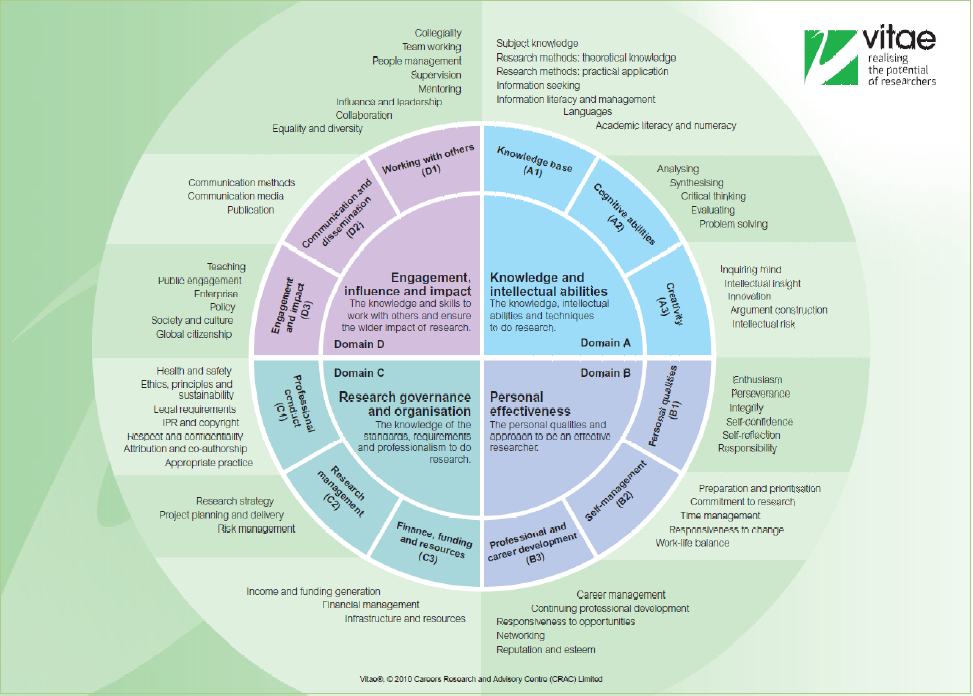
\includegraphics[width=0.8 \textwidth]{img/map.png}
  \end{center}
    \end{block}
  }

  
   \frame{
   \frametitle{}
  \begin{block}{\begin{center}
Gráficos en publicaciones, informes, presentaciones...                 \end{center}}
   \begin{center}
    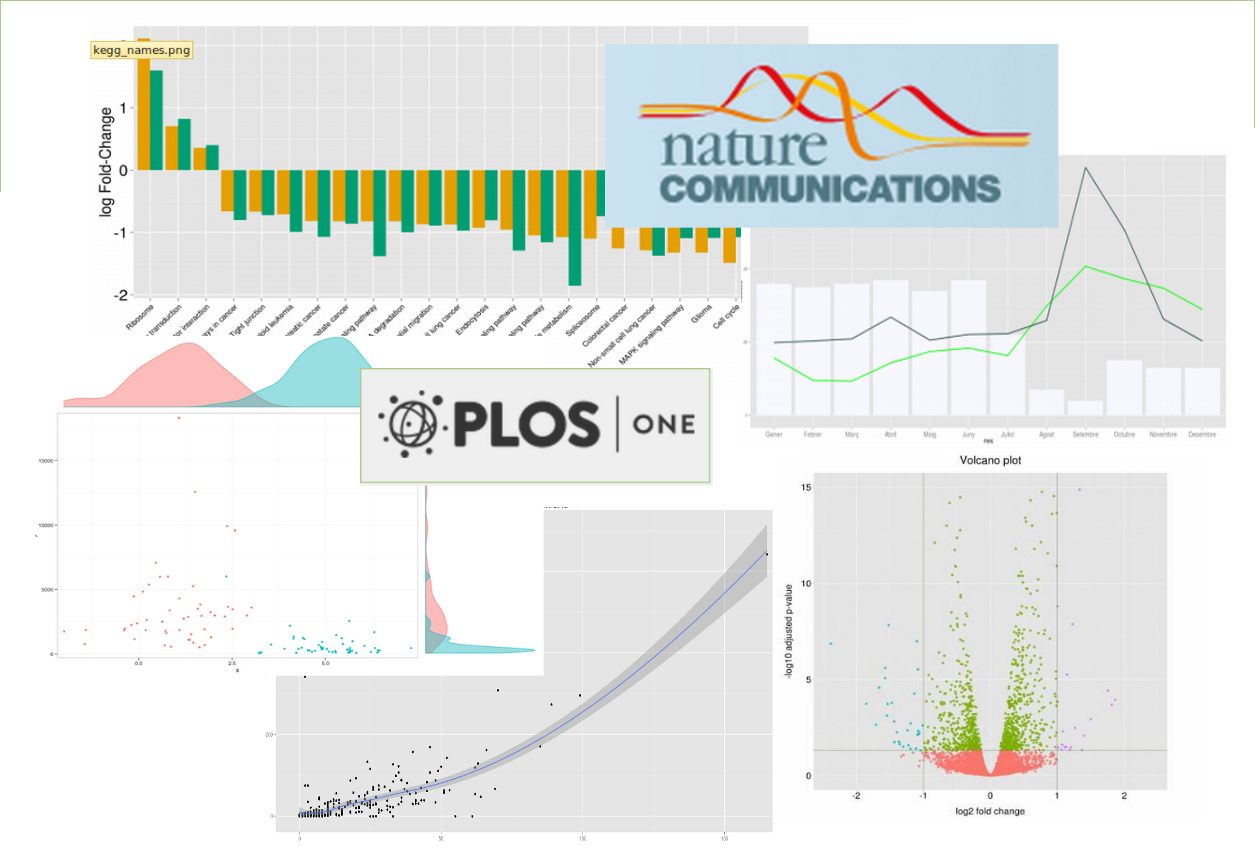
\includegraphics[width=0.9\textwidth]{img/plots.png}
  \end{center}
    \end{block}
  }

  
  \frame{
   \frametitle{}
  \begin{block}{¿Qué recursos utilizaremos para generar gráficos?}
    \begin{itemize}
       \vspace{4mm}
       \item  Excel, Power-Point.... no las utilizaremos porque ya las conocéis ;)
       \vspace{4mm}
       \item \lstinline {R} es una potente \textbf{herramienta de análisis estadístico y producción de gráficos}.
       \vspace{4mm}
       \item \textbf{Herramientas web }que representan gráficamente los resultados obtenidos en distintos análisis estadísticos.
       \vspace{4mm}
       \item Esta sesión está  relacionada con la que ofrecerá Ibo Galindo sobre la \textbf{imagen digital en investigación y publicación científica}.
       \vspace{4mm}
       \end{itemize}
  \end{block}
   }
  
 

%----------------------------------------------------------------------------
\section[Gráficos con R]{Gráficos con R} 

\subsection{¿Qué es \lstinline {R}?} 

\frame{
   \frametitle{}
  \begin{block}{¿Qué es \lstinline {R}?}
    \begin{itemize}
       \item \lstinline {R} es un entorno de programación que permite hacer análisis estadísticos.
       \vspace{1mm}
       \item Es una potente herramienta para generar gráficos de cualquier tipo. 
       \vspace{1mm}
       \item \lstinline {R}  es de código abierto y pertenece al proyecto GNU de software libre.
       \vspace{1mm}
        \item Disponible para las plataformas Linux, Macintosh y Windows.
       \vspace{1mm}
       \item \lstinline {R} es un software orientado tanto a usuarios principiantes com profesionales e investigadores que necesiten analizar y representar gráficamente sus datos.
       \vspace{1mm}
       \item \lstinline {R} es gratuito. No necesitamos ningún tipo de licencia.
       \vspace{1mm}
     \end{itemize}
  \end{block}
   }

\frame{
   \frametitle{}
  \begin{block}{¿Cómo obtenemos e instalamos  \lstinline {R}?} 
    \begin{itemize}
       \item Descargamos \lstinline {R} en \href{http://cran.r-project.org/}{http://cran.r-project.org/}
       \vspace{1mm}
       \item Tras la descarga, ejecutamos el archivo y aparecerá un asistente que nos guiará en el proceso. En unos minutos el software quedará instalado. 
       \vspace{1mm}
       \item Va bien instalarse \textbf{RStudio}, un interfaz que facilita el trabajo con \lstinline {R}. Está disponible en   \href{http://www.rstudio.com/}{http://www.rstudio.com/}
       \vspace{1mm}
        \item También hay disponible una versión libre. El modo de instalación es similar: descargamos la herramienta y la instalamos siguiendo el asistente. 
       \vspace{1mm}
       \item De modo que podemos trabajar directamente desde \lstinline {R} o bien desde \textbf{RStudio}. 
       \vspace{1mm}
       \end{itemize}
  \end{block}
   }


\subsection {Ejemplos y ejercicios}

\frame{
   \frametitle{}
  \begin{block}{Vamos a por la primera sesión de \lstinline {R}}
    \begin{itemize}
       \vspace{1mm}
       \item Abrimos \lstinline {R} 
       \vspace{1mm}
       \item También abrimos este documento con ejemplos y ejercicios: \href{http://fgardos.github.io/graficos_estadisticos_1.html}{\textbf{enlace}}
       \vspace{1mm}
       \item Para cada gráfico ejecutamos sus respectivos comandos e intentamos asociar qué es lo que hace cada uno de ellos.
       \vspace{1mm}
        \item Al final del documento, hay unos ejercicios que nos están esperando.
       \vspace{1mm}
       \end{itemize}
  \end{block}
   }





%----------------------------------------------------------------------------
\section[Herramientas web]{Herramientas web} 

  \frame{
   \frametitle{}
  \begin{block}{Herramientas web}
    \begin{itemize}
       \vspace{3mm}
       \item Nos ayudan a representar y visualizar los resultados de un análisis estadístico en un entorno biológico. 
       \vspace{3mm}
       \item Sólo necesitamos un navegador web para acceder a la herramienta y nuestros datos.
       \vspace{3mm}
       \item Veremos algunas ideas básicas sobre Paintomics, Babelomics, CellMaps.   
       \vspace{3mm}
       \end{itemize}
  \end{block}
   }



\subsection {Paintomics}
  
  \frame{
   \frametitle{}
  \begin{block}{Paintomics}
    \begin{itemize}
       \vspace{3mm}
       \item Es una herramienta de integración y visualización de datos ómicos.
       \vspace{3mm}
       \item El \textbf{input} es el resultado que hemos obtenido en un análisis de datos transcriptómicos y metabolómicos. 
       \vspace{3mm}
       \item El \textbf{output} es la representación gráfica de pathways de señalización (\href{http://www.genome.jp/kegg/}{\textbf{KEGG}}), incluyendo los datos proporcionados anteriormente.  
       \vspace{3mm}
              \item \textbf{Tutorial:} \href{http://www.paintomics.org/userguide/index.html}{http://www.paintomics.org/userguide/index.html}
        \vspace{3mm}
       \end{itemize}
  \end{block}
   }

   
   
 \frame{
   \frametitle{}
  \begin{block}{\begin{center} Input    \end{center}}
   \begin{center}
    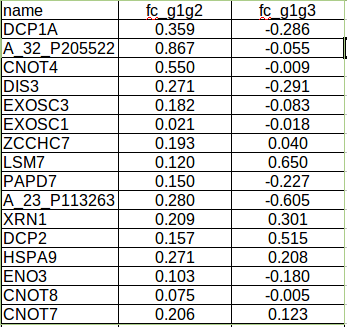
\includegraphics[width=0.6 \textwidth]{img/painto1.png}
  \end{center}
    \end{block}
  }
  
   \frame{
   \frametitle{}
  \begin{block}{\begin{center} Output    \end{center}}
   \begin{center}
    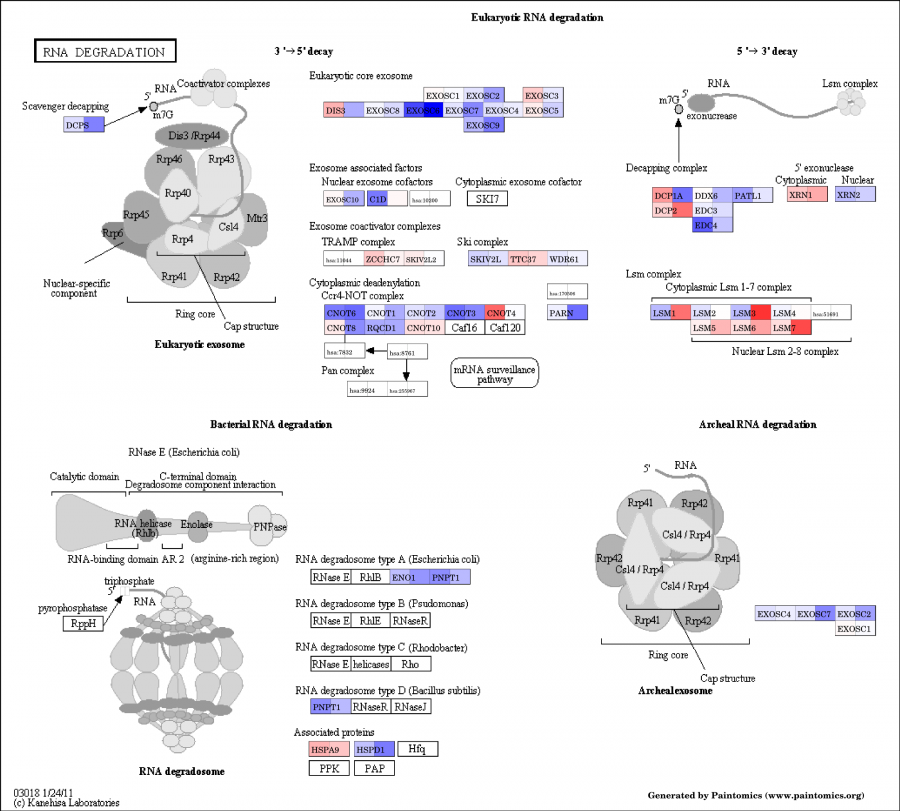
\includegraphics[width=0.6 \textwidth]{img/painto2.png}
  \end{center}
 \begin{center}
 Vamos a trabajar con  la herramienta: \href{http://www.paintomics.org/cgi-bin/main2.cgi}{\textbf{Paintomics}}                                                                                                               \end{center}
    \end{block}
  }



  
  \subsection {Babelomics}

\frame{
   \frametitle{}
  \begin{block}{Babelomics}
    \begin{itemize}
       \vspace{3mm}
       \item Es una herramienta de análisis de datos transcriptómicos, proteómicos,... También para cualquier grupo de datos biológicos o clínicos.   
       \vspace{3mm}
       \item \textbf{Input:} son ficheros de texto que incluyen datos en formato rectangular o matricial. 
       \vspace{3mm}
       \item  \textbf{Output:} gráficos: heatmaps, árboles de clustering, gráficos de análisis de componentes principales,...
       \vspace{3mm}
       \item \textbf{Tutorial:} \href{http://bioinfo.cipf.es/babelomicstutorial/}{http://bioinfo.cipf.es/babelomicstutorial/}
        \vspace{3mm}
       \end{itemize}
  \end{block}
   }
   
    \frame{
   \frametitle{}
  \begin{block}{\begin{center} Input    \end{center}}
   \begin{center}
    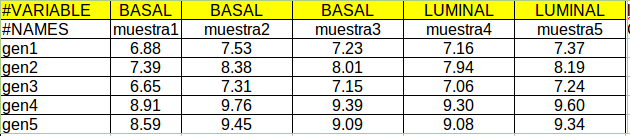
\includegraphics[width=1 \textwidth]{img/babel1.png}
  \end{center}
    \end{block}
  }
  
   \frame{
   \frametitle{}
  \begin{block}{\begin{center} Output: heatmap con diferencias entre grupos    \end{center}}
   \begin{center}
    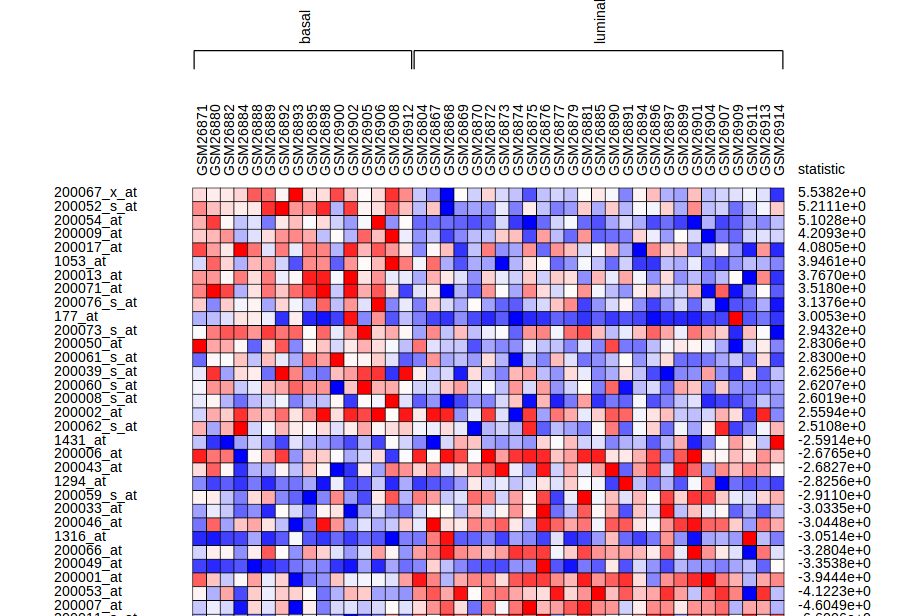
\includegraphics[width=0.8 \textwidth]{img/babel2.png}
  \end{center}
    \end{block}
  }
  
    \frame{
   \frametitle{}
  \begin{block}{\begin{center} Output: clustering de individuos  \end{center}}
   \begin{center}
    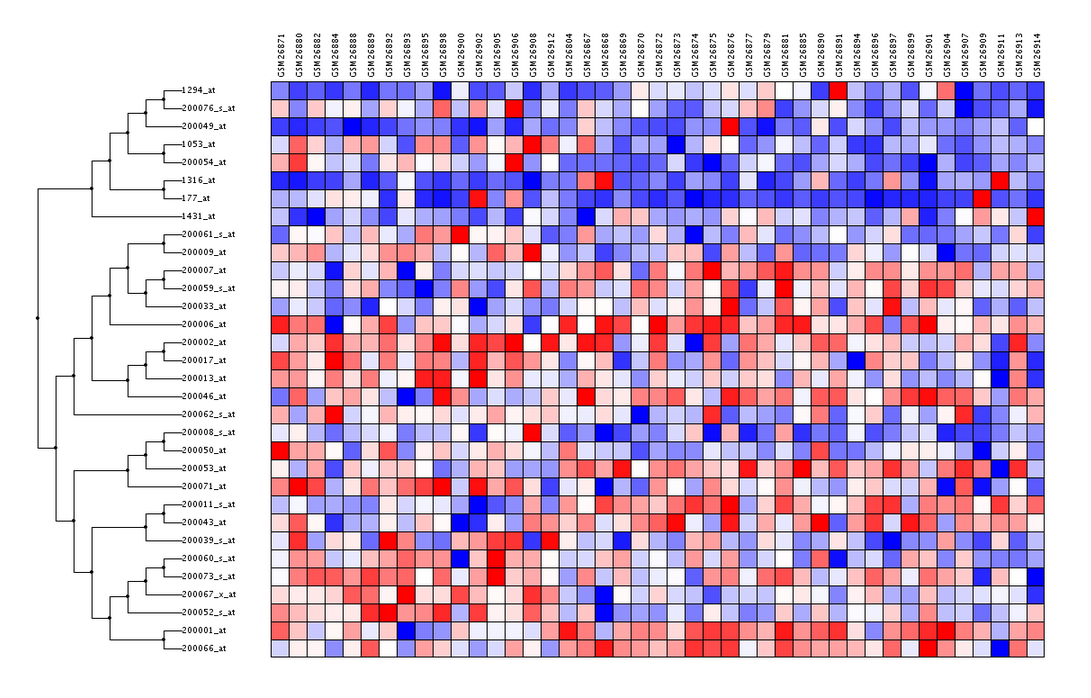
\includegraphics[width=0.8 \textwidth]{img/babel3.png}
  \end{center}
 \begin{center}
 Vamos a trabajar con  la herramienta: \href{http://babelomics.bioinfo.cipf.es/}{\textbf{Babelomics}}                                                                                                               \end{center}
    \end{block}
  }
 
  
  \subsection {CellMaps}

\frame{
   \frametitle{}
  \begin{block}{CellMaps}
    \begin{itemize}
       \vspace{3mm}
       \item Es una herramienta que permite la integración, visualización y el análisis de \textbf{redes biológicas}.   
       \vspace{3mm}
       \item El \textbf{input} es un fichero donde indicamos las relaciones entre los nodos de nuetra red. Opcionalmente podemos incluir un fichero con los \textbf{atributos} de cada nodo.
       \vspace{3mm}
       \item El \textbf{output} gráfico es una red en la que se muestran las relaciones de los distintos nodos que la integran. Simultáneamente es posible  visualizar los atributos de los elementos biológicos de la red. 
       \vspace{3mm}
       \item \textbf{Tutorial:} \href{https://github.com/opencb/cell-maps/wiki}{https://github.com/opencb/cell-maps/wiki}
        \vspace{3mm}
       \end{itemize}
  \end{block}
   }
   
   
   \frame{
   \frametitle{}
  \begin{block}{\begin{center} Input    \end{center}}
   \begin{center}
    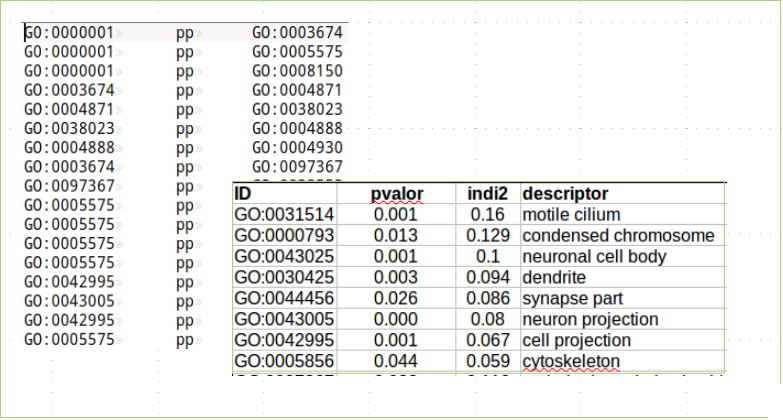
\includegraphics[width=0.9 \textwidth]{img/cellmaps1.png}
  \end{center}
    \end{block}
  }
  
   \frame{
   \frametitle{}
  \begin{block}{\begin{center} Output    \end{center}}
   \begin{center}
    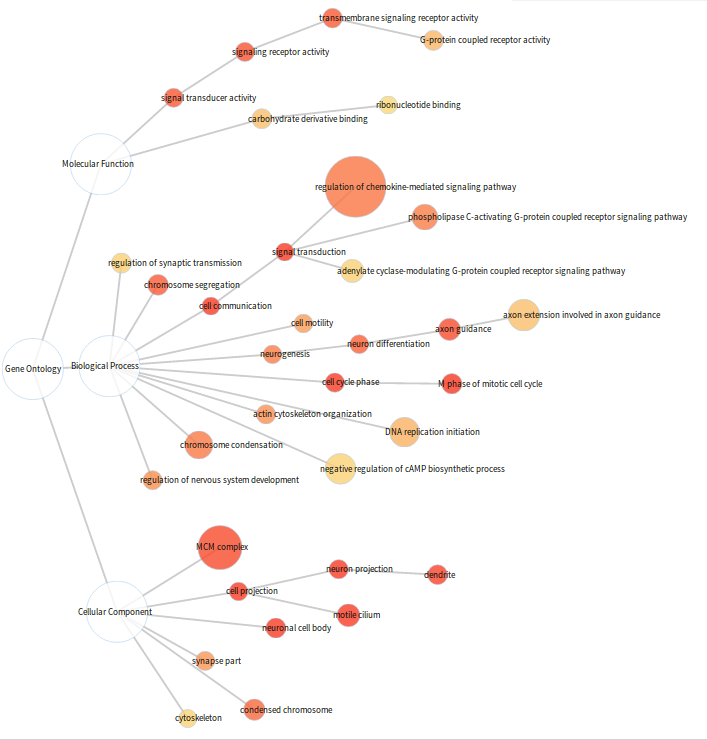
\includegraphics[width=0.5 \textwidth]{img/cellmaps2.png}
  \end{center}
 \begin{center}
 Vamos a trabajar con  la herramienta: \href{http://cellmaps.babelomics.org/}{\textbf{Cellmaps}}                                                                                                               \end{center}
    \end{block}
  }


  
   \frame{
   \frametitle{}
  \begin{block}{}
   \begin{center}
    
\includegraphics[width=0.5 \textwidth]{img/questions.png}
  \end{center}
    \end{block}
  }  
  
\end{document}
